\documentclass[12pt,letterpaper]{article}

\usepackage{amsmath, amsthm, amsfonts, amssymb}
\usepackage{graphicx,hyperref}
\usepackage{microtype, parskip}
\usepackage[numbers,sort&compress]{natbib}
\usepackage{lineno}
\usepackage{docmute}
\usepackage[font=small]{caption}
\usepackage{subcaption, multirow, morefloats}
\usepackage{wrapfig, rotating}
\usepackage{titlesec}
\usepackage{authblk, attrib, fullpage}
\usepackage{lineno}

\frenchspacing

\captionsetup[subfigure]{position = top, labelfont = bf, textfont = normalfont, singlelinecheck = off, justification = raggedright}

\begin{document}
\section{Methods}

\subsection{Species information}

Fossil occurrence information was downloaded from the Paleobiology Database (PBDB; \url{http://paleodb.org/}). Occurrence, taxonomic, stratigraphic, and biological information was downloaded for all North American mammals. This data set was filtered so that only occurrences identified to the species level, excluding all ``sp.''-s. All aquatic and volant taxa were also excluded. Additionally, all occurrences without latitude and longitude information were excluded.

Species dietary and locomotor category assignments were done using the assignments in initial the PBDB which were then reassigned into coarser categories (Table \ref{tab:trait_cats}). This was done to improve interpretability, increase sample size per category, and make these results comparable to previous studies \citep{Jernvall2004,Price2012}.

\begin{table}
  \centering
  \caption{Species trait assignments in this study are a coarser version of the information available in the PBDB. Information was coarsened to improve per category sample size and uniformity and followed this table.}
  \begin{tabular}[ht]{ l | l | l }
    \hline
    \multicolumn{2}{ c |}{This study} & PBDB categories \\
    \hline \hline
    \multirow{4}{*}{Diet} & Carnivore & Carnivore \\
    & Herbivore & Browser, folivore, granivore, grazer, herbivore. \\
    & Insectivore & Insectivore. \\
    & Omnivore & Frugivore, omnivore. \\ 
    \hline
    \multirow{3}{*}{Locomotor} & Arboreal & Arboreal.\\
    & Ground dwelling & Fossorial, ground dwelling, semifossorial, saltatorial. \\
    & Scansorial & Scansorial. \\
    \hline
  \end{tabular}
  \label{tab:trait_cats}
\end{table}


Fossil occurrences were assigned to 2 My bins ranging through the entire Cenozoic. Taxon duration was measured as the number of bins from the first bin of occurrence to the last bin of occurrence, inclusive.

Species body size estimates were sourced from a large selection of primary literature and compilations, principally the PBDB, PanTHERIA \citep{Jones2009c}, the Neogene Old World Mammal database (Now; \url{http://www.helsinki.fi/science/now/}), and other large scale data collection efforts \citep{Smith2004c, Raia2012f, Brook2004a, Freudenthal2013, McKenna2011}. In many cases, species body mass was estimated from anatomical dimensions such as tooth size. These estimates were made using a variety of published regression equations. See Appendix: Data for a complete list of individual sources and equations. % equations in a giant table/appendix section


\subsubsection{Bioprovince occupancy}

For each 2 My time bin, a bipartite biogeographic network was created between species occurrences and spatial units. Spatial units were defined was 2x2 latitude--longitude grid cells from an azimuthal equal-area map projection. In these bipartite networks, taxa can only be linked to localities and \textit{vice versa}. Taxa are not linked to each other, nor are localities linked. Emergent bioprovinces within the biogeographic occurrence network were identified using the map equation \citep{Rosvall2008,Rosvall2009a}. A bioprovince is a set of species--locality connections that are more interconnected within the group than without. This was done for each bin's biogeographic network using the \texttt{igraph} package for R \citep{csardi2006igraph,2014language}. The relative number of bioprovinces occupied per time bin was then determined for each species. %Additionally, the coefficient of variation (CV) of occupancy was also calculated.


\subsubsection{Semi-formal supertree}

Because there exists no phylogenetic hypothesis of all Cenozoic fossils mammals from North America, it was necessary to construct a semi-formal supertree. This was done by combining taxonomic information for all the observed species and a few published phylogenies.

The taxonomic information from the PBDB served as the basis for additional revision. The taxonomy of many species was updated using the Encyclopedia of Life (\url{http://eol.org/}), which collects and collates taxonomic information in a single database. This was done programatically using the \texttt{taxize} package for R \citep{2013taxize}. This was additionally correct using various published phylogenies and taxonomies of fossil mammals \citep{Raia2012f,Janis1998,Janis2008}, producing a tree that was a series of nested polytomies. 
%Using the \texttt{treebase} package for R \citep{boettiger2014treebase}, I downloaded all phylogenies where at least one of the observed fossil taxon was sampled. 
%MRP supertree implemented in the \texttt{phytools} package for R \citep{revell2012phytools}

Polytomies were resolved in order of species first appearance. The resulting tree was then time scaled using the \texttt{paleotree} package via the ``minimum branch length'' approach with a minimum length of 0.1 My \citep{Bapst2012a}. The minimum length is necessary to avoid zero-length branches which cause the phylogenetic covariance matrix not be positive definite, which is an important convenience for computation (see below). While other time scaling approaches are possible \citep{Bapst2013a,Hedman2010} this method was chosen for it's simplicity and not requiring additional information about diversification rates which are of interest in this study. 
% I really wish I was using the Hedman approach.



\subsection{Survival model}

The statistical model described here was the final model at the end of a continuous model development framework where the sampling and prior distributions were iteratively modified to best reflect theory, knowledge of the data, the inclusion of important covariates, and to fit the data. This follows the approach described in \citet{Gelman2007} and \citet{Gelman2013d}.
A survival model was fit in a Bayesian context where species duration were assumed to be drawn from a Wiebull distribution (Eq. \ref{eq:weibull}) with shape \(\alpha\) and scale \(\sigma\) parameters. 
\begin{align}
  p(y_{i}|\alpha, \sigma) &= \mathrm{Weibull}(y_{i}|\alpha, \sigma) \nonumber \\ 
  &= \frac{\alpha}{\sigma} \left(\frac{y_{i}}{\sigma}\right)^{\alpha - 1} \exp\left(-\left(\frac{y_{i}}{\sigma}\right)^{\alpha}\right) 
  \label{eq:weibull}
\end{align}

Following standard practice in survival analysis \citep{Klein2003}, \(\alpha\) was assumed constant and was given a weakly informative half-Cauchy prior. 
% Should I give this a much stronger prior? 
% Hierarchical modeling of \alpha would be a pain in the ass, but potentially illuminating.
\(\sigma\) was reparameterized as an exponentiated regression model (Eq. \ref{eq:reg}). Note, the inclusion of \(\alpha\) in the denominator of the exponentiated term is a standard parameterization for survival models using a Wiebull distribution \citep{Klein2003}.

\begin{equation}
  \sigma = \exp\left(\frac{-(h_{i} + \eta_{j[i]} + \sum \beta^{T} \mathbf{X}_{i})}{\alpha}\right)
  \label{eq:reg}
\end{equation}

\(K\) species level covariates were included as a \(n \times K\) matrix, \(\mathbf{X}\). The covariates of interest included the logit of mean relative occupancy and the logarithm of body size (g). The discrete covariate index variables dietary and locomotor category were transformed into \(n \times (k - 1)\) matrices where each column is an indicator variable (0/1) for that species's category, \(k\) being the number of categories of the index variable. Only \(k - 1\) indicator variables are necessary as the intercept takes on the remaining value. Finally, a vector of 1-s were included in the matrix \(\mathbf{X}\) whose corresponding \(\beta\) coefficient is the intercept, making \(K\) equal eight.

\(\beta\) is a vector of regression coefficients, where each element was given a unique, weakly informative Normally distributed prior. These priors were chosen because it is expected that the effect size of each variable on duration will be small, as is generally the case with binary covariates. %In all cases, posterior inference was not effected by changes to this choice of prior. Do I have proof?

Regression coefficients are not directly comparable without first standardizing the input variables to have equal standard deviations. This linear transform greatly improves the interpretability of the coefficients as expected change in mean duration given a difference of one standard deviation in the covariate \citep{Schielzeth2010}. However, because the expected standard deviation for a binary variable is 0.5, in order to make comparisons between the binary and continuous variables, the continuous inputs were divided by twice their standard deviation \citep{Gelman2008}. The above model was fit with both unstandardardized and standardized inputs for illustrative purposes.


\subsubsection{Hierarchical effects}

The two hierarchical effects of interest in this study are origination cohort and shared evolutionary history, or phylogeny. Hierarchical modeling can be considered an intermediate between complete and no pooling \citep{Gelman2007}, where complete pooling is when the differences between groups are ignored while no pooling is where different groups are analyzed separately. By allowing for partial pooling, we are modeling a compromise between these two extremes which allows for better inference. This is done by having all of the groups sharing the same prior with the scale parameter estimated from the data, which then acts as an indicator of the amount of pooling. A scale of 0 and \(\infty\) indicate complete and no pooling, respectively. Hierarchical modeling is analogous to mixed-effects modeling \citep{Gelman2007}. 

Origination cohort is defined as the group of species which originated during the same 2 My temporal bin. The most recent temporal bin, 0-2 Mya, was excluded, leaving 32 different cohorts. The effect of origination cohort \(j\) was modeled with each group being a sample from a common cohort effect, \(\eta\), which was considered Normally distributed with mean 0, and standard deviation \(\sigma_{c}\). The value of \(\sigma_{c}\) was then estimated from the data itself, corresponding to the amount of pooling in the individual estimates of \(\eta_{j}\). This approach is a conceptual unification between dynamic and cohort survival analysis in paleontology \citep{Foote1988,Raup1978,Raup1975,VanValen1979,Baumiller1993}, with \(\sigma_{c}\) acting as a measure of relative importance of these two end members.

\begin{align*}
  \eta_{j} &\sim \mathcal{N}(0, \sigma_{c}) \\
  \sigma_{c} &\sim \mathrm{halfCauchy}(0, 2.5)
\end{align*}

The choice of prior for \(\sigma_{c}\) follows \citet{Gelman2006a}

The impact of shared evolutionary history, or phylogeny, was modeling as an individual effect where each observation, \(i\), is distributed as a multivariate normal, \(h\), where the covariance matrix was assumed known up to a constant variance, \(\sigma_{p}^{2}\) \citep{Lynch1991,Housworth2004}. More fully, this is written

\begin{align*}
  h &\sim \mathrm{Multi}\mathcal{N}(0, \mathbf{\Sigma}) \\
  \mathbf{\Sigma} &= \sigma_{p}^{2} \mathbf{V}_{phy} \\
  \sigma_{p} &\sim \mathrm{halfCauchy}(0, 2.5),
\end{align*}
 
with \(\mathbf{V}_{phy}\) being the phylogenetic covariance matrix defined as an \(n \times n\) matrix where the diagonal elements are the distance from root to tip, in branch length, for each observation and the off-diagonal elements are the amount of shared history, measured in branch length, between observations \(i\) and \(j\). \(\sigma_{p}\) was given a weakly informative half-Cauchy hyperprior. 

Both \(\eta\) and \(h\) were centered at 0 so that these effects can be interpreted as differences from the mean of the observed.


\subsubsection{Censored observations} \label{sec:censor}

An important part of survival analysis is the inclusion of ``censored'' observations \citep{Ibrahim2001,Klein2003} or observations where the failure time has not been observed. The most common censored observation is right censored, where the point of extinction had not yet been observed in the period of study. In this case, this means taxa that are still extant. Left censored observations, on the other hand, correspond to observations that went extinct any time between 0 and some known point. In this study, taxa occurring in only a single time bin were left censored. Because of the minimum resolution of the record, we cannot observe if these taxa went extinct in less than that single bin or not. 

To model censored data, there are a few functions which must first be defined following \citet{Klein2003}. The survival function, \(S(t)\), for a Weibull model is
\begin{equation}
  S(t | \alpha, \sigma) = \exp\left(-\left(\frac{t}{\sigma}\right)^{\alpha}\right),
  \label{eq:surv}
\end{equation}
where \(\sigma\) is defined as above (Eq. \ref{eq:reg}). \(S(t)\) is the probability that an observation will survive longer than a give time, \(t\). The likelihood of uncensored observations is evaluated as as normal using Equation \ref{eq:weibull} while right censored observations are evaluated at \(S(t)\) and left censored observations are evaluated at \(1 - S(t)\). Note, \(1 - S(t)\) is equivalent to the cummulative density function and \(S(t)\) is equivalent to the complementary cummulative density function \citep{Gelman2013d}.

Fully, the likelihood for both uncensored and both right and left censored observations is written
\begin{equation*}
  L \propto \prod_{i \in C} \mathrm{Weibull}(y_{i} | \alpha, \sigma) \prod_{j \in R} S(y_j | \alpha, \sigma) \prod_{k \in L} \left(1 - S(y_{k} | \alpha, \sigma)\right),
\end{equation*}
where \(C\) is the set of uncensored observations, \(R\) is the set of right censored observations, and \(L\) is the set of left censored observations.

A summary of the entire model, save for calculations for censored observations, along with the exact priors for every estimated parameter is presented in Figure \ref{fig:model_diagram}.

\begin{figure}
  \centering
  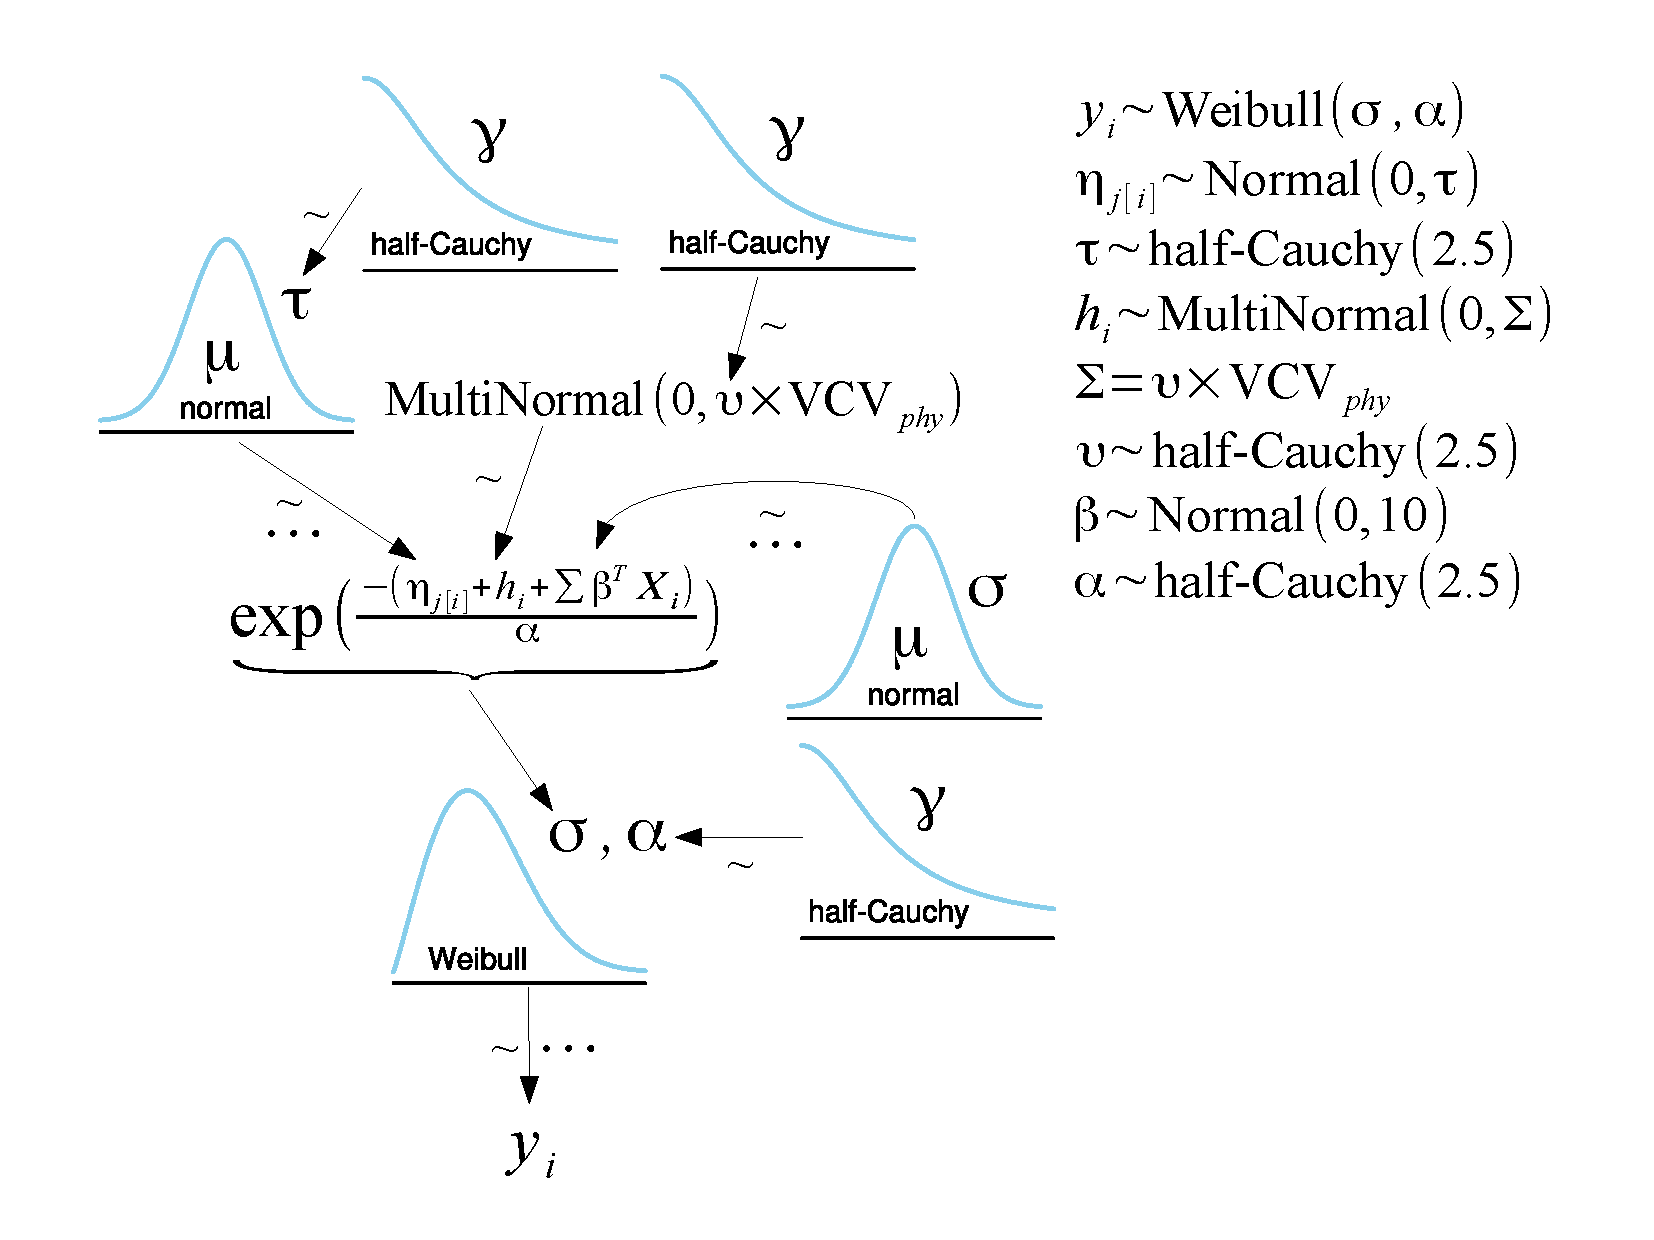
\includegraphics[height = 0.5\textheight, width = \textwidth, keepaspectratio = true]{figure/mammal_survival_model}
  \caption{Graphical depiction of full survival model, save censoring, used here. Exact values for the hyperparameters are presented to the right. The observed duration of the \(i\)th observation is indicated towards the bottom left as \(y_{i}\), which is assumed to follow a Weibull distribution.}
  \label{fig:model_diagram}
\end{figure}


\subsubsection{Estimation}
Parameter posteriors were approximated using a Markov-chain Monte Carlo (MCMC) routine implemented in the Stan programming language \citep{2014stan}. Stan implements a Hamiltonian Monte Carlo using a No-U-Turn sampler \citep{Hoffman-Gelman:2011}. Posterior approximation was done using four parallel MCMC chains. Chain convergence was evaluated using the scale reduction factor, \(\hat{R}\). Values of \(\hat{R}\) close to 1, or less than or equal to 1.1, indicate approximate convergence. Convergence means that the chains are approximately stationary and the samples are well mixed \citep{Gelman2013d}.

Both models with and without phylogenetic effects were estimated. Because inverting a large matrix is a memory intense procedure and because the phylogenetic covariance matrix is only assumed known up to a constant, every iteration of the MCMC would involve solving a very large matrix which is not ideal. In order to speed up the MCMC routine, this aspect of the model had to be reparameterized for efficiency purposes. Because of the size of the covariance matrix a custom multivariate sampler was used (see Appendix: Code).

For the model without phylogenetic effect the four MCMC chains ran for 1000 steps, with the first 500 used as warm-up and the last 500 as samples from the posterior. Because of the added complexity of estimating the phylogenetic effect, instead all four chains were run 20000 steps thinned to every twentieth sample split evenly between warm-up and sampling. 



\subsection{Posterior predictive checks}

The most basic assessment of model fit is that simulated data generated using the fitted model should be similar to the observed. This is the idea behind posterior predictive checks. Using the predictors from each of the observed durations, and randomly drawn parameter estimates from their marginal posteriors, a simulated data set \(y^{rep}\) was generated. This process repeated 1000 times and the distribution of \(y^{rep}\) was compared with the observed \(y\) \citep{Gelman2013d}. This was done both graphically and numerically.

An example posterior predictive check used in this study is a graphical comparison of the Kaplan-Meier (K-M) survival curve estimated from the observed data with the survival curves from 1000 simulations. K-M survival curves are non-parametric estimates of the function \(S(t)\) or the probability of a species going extinct given that it has lived to time \(t\) \citep{Klein2003}. Other posterior predictive checks included comparison of the mean and quantiles of the observed durations to the distributions of the same quantities from the simulations, and inspection of the deviance residuals, defined below.

In ordinary linear regression, the residuals are defined as \(r = y - y_{est}\). For hierarchical models, this definition is inadequate. For survival analysis, the equivalent values are deviance residuals. To define how deviance residuals are calculated, we first define the cummulative hazard function \citep{Klein2003}. Given \(S(t)\) (Eq. \ref{eq:surv}), we define the cumulative hazard function as 
\begin{equation*}
  \Lambda(t) = -log\left(S\left(t\right)\right).
\end{equation*}

Next, we define martingale residuals, \(m\), which are defined in relation to the inclusion vector \(I\)
\begin{equation*}
  m_{i} = I_{i} - \Lambda(t_i).
\end{equation*}
\(I\) is as a vector of length \(n\), where \(I_{i} = 1\) means the observation is completely observed and \(I_{i} = 0\) means the observation is censored. 

Martingale residuals have a mean of 0 and ranges between 1 and \(-\infty\) and can be viewed as the difference between the observed number of deaths between 0 and \(t_{i}\) and the expected number of deaths based on the model. However, martingale residuals are difficult to interpret, can be asymmetrically distributed, and are not equivalent to standard residuals. 

The solution to this is to use the deviance residuals, \(D\). This is defined as a function of martingale residuals and takes the form
\begin{equation*}
  D_{i} = \text{sign}(m_{i}) \sqrt{-2[m_{i} + I_{i}log(I_{i} - m_{i})]}.
\end{equation*}


\subsection{Variance partitioning}
There are three different variance components in this model (Fig. \ref{fig:model_diagram}): sample \(\sigma_{y}^{2}\), cohort \(\sigma_{c}^{2}\), and phylogenetic \(\sigma_{p}^{2}\). The sample variance, \(\sigma_{y}^{2}\), is similar to the residual variance from a normal linear regression. Partitioning the variance between these sources allows the relative amount of unexplained variance of the sample to be compared. However, the model used here (Eq. \ref{eq:weibull}) does not include an estimate of overall variance, as the errors are not normally distributed. The partitioning of the variance between these three components was instead approximated via a simulation approach modified from \citet{Goldstein2002}.

The procedure is as follows:
\begin{enumerate}
  \item Simulate \(w\) (50,000) values of \(\eta\); \(\eta \sim \mathcal{N}(0, \sigma_{c})\).
  \item For a given value of \(\beta^{T} \mathbf{X}\), calculate \(\sigma^{c*}\) (Eq. \ref{eq:reg}) for all \(w\) simulations, holding \(h\) constant at 0.
  \item Calculate \(\upsilon_{c}\), the Weibull variance (Eq. \ref{eq:wei_var}) of each element of \(\sigma^{c*}\) with \(\alpha\) drawn from the posterior estimate.
  \item Simulate \(w\) values of \(h\); \(h \sim \mathcal{N}(0, \sigma_{p})\)
  \item For a given value of \(\beta^{T} \mathbf{X}\), calculate \(\sigma^{p*}\) (Eq. \ref{eq:reg}) for all \(w\) simulations, holding \(\eta\) constant at 0.
  \item Calculate \(\upsilon_{p}\), the Weibull variance (Eq. \ref{eq:wei_var}) of each element of \(\sigma^{p*}\) with \(\alpha\) drawn from the posterior estimate.
  \item \(\sigma_{y*}^{2} = \frac{1}{2} \left(\left(\frac{1}{w} \sum_{i}^{w} \upsilon_{pi}\right) + \left(\frac{1}{w} \sum_{j}^{w} \upsilon_{cj}\right)\right)\)
  \item \(\sigma_{c*}^{2} = var(\upsilon_{c})\) and \(\sigma_{p*}^{2} = var(\upsilon_{p})\)
\end{enumerate}

The simulated values of \(h\) were drawn from a univariate normal distribution because each simulated value is in isolation, so there are is no concern of phylogenetic autocorrelation. The chosen value for \(\beta^{T} \mathbf{X}\) was a draw from the posterior estimate of the intercept. Because input variables were standardized prior to model fitting, the intercept corresponds to the estimated effect on survival of the sample mean.

Weibull variance is calculated as
\begin{equation}
  var(x) = \sigma^{2}\left(\Gamma\left(1 + \frac{2}{\alpha}\right) - \left(\Gamma\left(1 + \frac{1}{\alpha}\right)\right)^{2}\right),
  \label{eq:wei_var}
\end{equation}
where \(\Gamma\) is the gamma function. 

The variance partitioning coefficients are then calculated \(VPC_{phylo} = \frac{\sigma_{p*}^{2}}{\sigma_{y*}^{2} + \sigma_{c*}^{2} + \sigma_{p*}^{2}}\) and similar for the other variance components.

I used ratios of the variances and variance partitioning coefficients (VPC) to measure the amount of partial pooling. The former, when compared to the sample size of the hierarchical effect such as the number of cohorts, is an estimate of the relative amount of pooling, while the latter is a measure of the relative importance of the different variance components \citep{Gelman2007}. Phylogenetic heritability, \(h_{p}^{2}\) \citep{Housworth2004}, is effectively identical to the VPC of the phylogenetic effect. Additionally, because phylogenetic effect was estimated using a principally taxonomy based tree the estimates derived here can be considered minimum estimates of the tree effect.


\end{document}
